\chapter{Chạy local và trình diễn hệ thống}
\section{Cài đặt môi trường}
Người nhận giải nén toàn bộ thư mục Project01, cài Python 3.11 64-bit và mở terminal tại nơi có \texttt{app.py}. Mô hình, scaler, dữ liệu và KB đã được đóng gói; lần cài đầu chỉ cần tải thư viện. Sau đó demo suy luận có thể hoạt động không cần Internet hoặc API key.

\begin{lstlisting}[language={},caption={Tạo môi trường và khởi động bằng PowerShell.}]
py -3.11 -m venv .venv
.\.venv\Scripts\python.exe -m pip install --upgrade pip
.\.venv\Scripts\python.exe -m pip install torch==2.15.0 --index-url https://download.pytorch.org/whl/cpu
.\.venv\Scripts\python.exe -m pip install -r requirements.txt
.\.venv\Scripts\python.exe -m streamlit run app.py --server.address 127.0.0.1 --server.port 8521
\end{lstlisting}

Mở trình duyệt tại \url{http://127.0.0.1:8521}. Dừng server bằng Ctrl+C trong terminal. Có thể bấm đúp \texttt{run.cmd} để tự tạo môi trường và cài các thư viện ở lần đầu; script cần Python launcher có thể tìm Python 3.11. Nếu dùng Anaconda, tạo env Python 3.11, activate rồi gọi \texttt{python -m pip} và \texttt{python -m streamlit} với cùng tham số.

Gọi trực tiếp Python trong venv giúp tránh lỗi chính sách PowerShell đối với Activate.ps1. Server chỉ bind localhost; project chưa có cấu hình triển khai công khai, đăng nhập hay phân quyền. Khi port 8521 đang được dùng, đổi port và mở đúng URL mới.

\section{Các tab và luồng thao tác}
Giao diện dashboard có bốn tab. Hội chẩn demo có ba nút chạy nhanh, bảy thẻ trạng thái tác tử và vùng thiết lập hồ sơ/câu hỏi. Kết quả chia thành vòng điểm phân loại, các thẻ tri thức và hành động nhắc việc. Tri thức và đồ thị đặt ghi chú có URL cạnh bản đồ khái niệm. Thực nghiệm có biểu đồ tương tác để đổi giữa AUC, Average Precision và F1, cùng bảng/đường cong chi tiết. Hướng dẫn cung cấp các lệnh khởi chạy và tái lập.

Mặc định giao diện dùng hồ sơ mẫu lấy từ train. Người dùng chọn Nhập JSON để thay 21 chỉ báo, chọn tác vụ và bấm Bắt đầu phân tích. Mục Nhật ký và số đo chứa gap, fatigue và glucose bổ sung. Các thẻ tác tử chuyển màu theo thông điệp thực tế của phiên vừa chạy; chi tiết được thu gọn trong mục Chi tiết phối hợp tác tử.

\begin{figure}[H]\centering
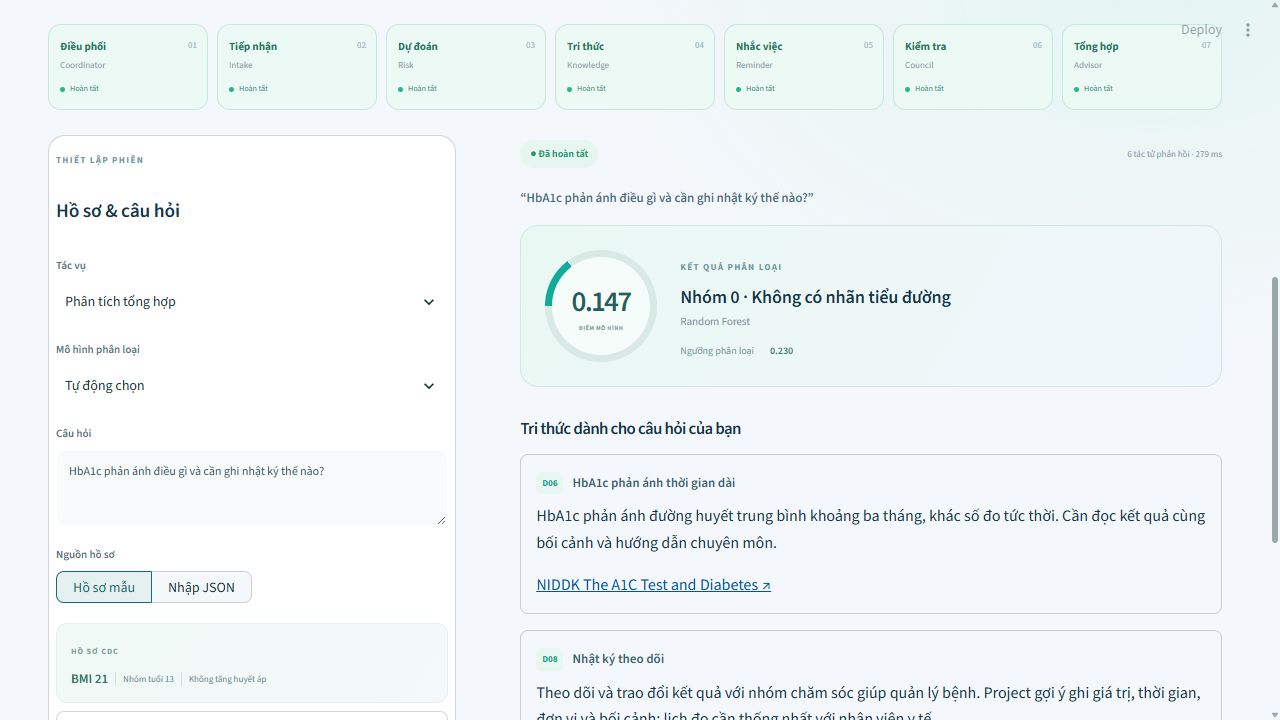
\includegraphics[width=\textwidth]{images/demo_consult.jpg}
\caption{Giao diện local sau khi chạy hội chẩn tổng hợp. Ảnh chụp từ trình duyệt của bản Project01.}
\end{figure}

\section{Ví dụ một lượt hội chẩn}
Với câu hỏi về HbA1c và nhật ký, hồ sơ train minh họa, gap bằng 2 và fatigue bằng 0, hệ thống nhận diện không có điều kiện dừng ở Intake. Risk chạy model mặc định Random Forest, Knowledge truy xuất các ghi chú liên quan và Reminder đọc Q-table seed 42. Council kiểm tra các proposal rồi Advisor ghép kết quả.

Ở hồ sơ minh họa được chọn, score Random Forest khoảng 0,147 và ngưỡng 0,230 nên dự đoán nhãn 0. Giao diện trình bày score bằng vòng điểm, kèm model và ngưỡng. Tri thức được tách thành các thẻ có ID/URL; hành động Reminder nằm trong thẻ nhắc nhật ký. Có thể tải kết quả của cả phiên bằng nút Tải kết quả phiên.

Trace có 12 thông điệp để người đọc thấy thứ tự gọi, trạng thái từng bước và thời gian. Có thể tải JSON để kiểm tra proposal, evidence và lý do duyệt. Bảng trace không phải chuỗi suy nghĩ ẩn của model; nó là log của những thao tác phần mềm thực sự đã gọi.

\begin{figure}[H]\centering
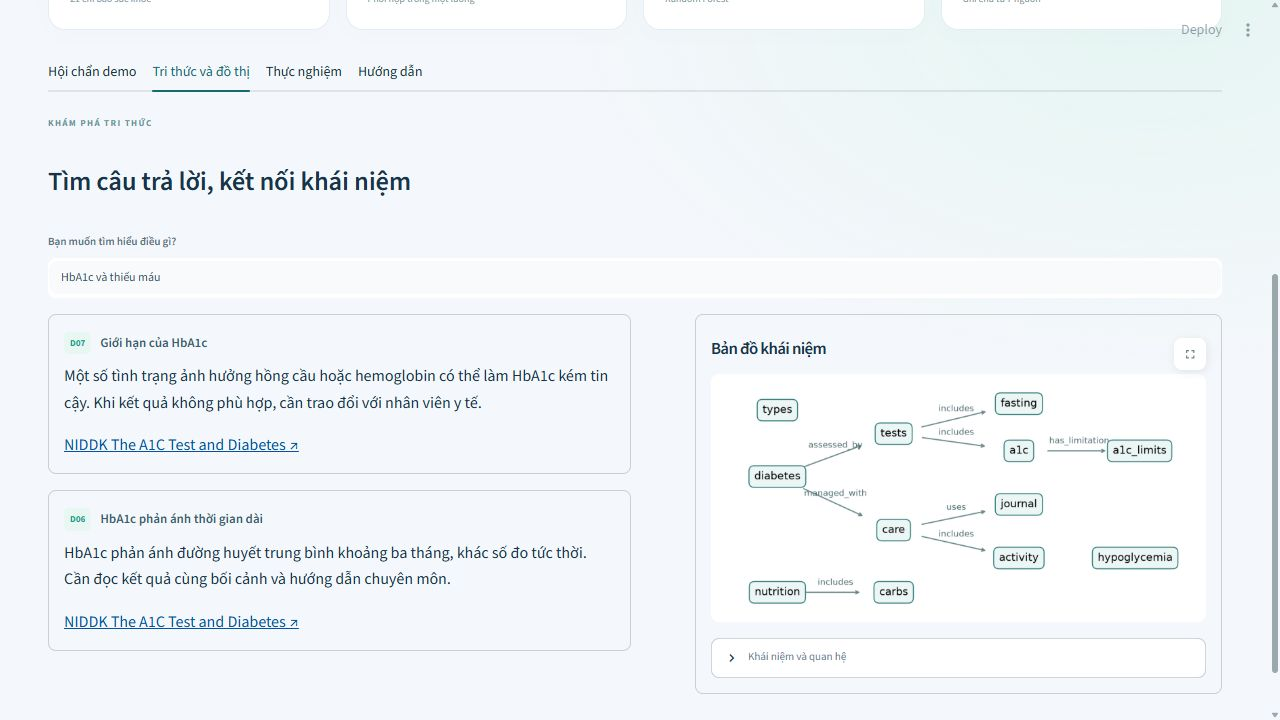
\includegraphics[width=\textwidth]{images/demo_knowledge.jpg}
\caption{Tab tri thức với query, ghi chú và URL nguồn để kiểm tra lại căn cứ.}
\end{figure}

\section{Kịch bản bảo vệ ngắn}
\begin{enumerate}[leftmargin=1.1cm]
\item Giới thiệu ba nhánh học sâu, tri thức và RL; nêu rõ phạm vi giáo dục.
\item Chạy hội chẩn mẫu, chỉ score/ngưỡng, đoạn có ID nguồn, reminder và 12 thông điệp.
\item Chọn riêng MLP; mở notebook 01 để nối từ kiến trúc tới output train và model đã lưu.
\item Hỏi về HbA1c và thiếu máu, mở nguồn của ghi chú; giải thích truy xuất và graph một bước.
\item Nhập hồ sơ chỉ có BMI để cho thấy needs\_input; sau đó thử số đo glucose 62 mg/dL để xem urgent trước Risk.
\item Mở kết quả RL, nêu trung thực Q-learning chưa vượt fixed. Dùng notebook 04 để trình diễn Council bác proposal thuốc hoặc ID giả.
\end{enumerate}
Tài liệu \texttt{docs/KICH\_BAN\_DEMO.md} phân bổ khoảng tám phút cho các thao tác trên. Không dùng hồ sơ thật hoặc nhập thông tin riêng tư khi bảo vệ.

\section{Tái lập thực nghiệm và notebook}
\begin{lstlisting}[language={},caption={Các lệnh tái lập độc lập với giao diện.}]
python scripts/run_experiments.py
python scripts/execute_notebooks.py
python -m pytest -q --junitxml=artifacts/test-results.xml
python scripts/update_report_assets.py
\end{lstlisting}

Các lệnh cần chạy bằng Python của môi trường đã cài dependencies. Script experiment có thể chạy riêng stage models, rl hoặc evaluation. Notebook 01 và 03 train thật nên khi Run All sẽ ghi lại artifact. Không nên mở quá trình train cùng lúc với demo vì app có thể đọc file trong lúc đang ghi. Sau train, khởi động lại app để nạp model mới.

Nếu muốn dùng Jupyter tương tác, chạy \texttt{python -m notebook}, mở theo thứ tự 01--04 và chọn đúng kernel. Mỗi notebook bắt đầu bằng cell in phiên bản Python và xác định thư mục project. Script build\_notebooks chỉ dùng để bảo trì phần source notebook, không tạo output thực và sẽ xóa output cũ nếu chạy lại.

\section{Xử lý lỗi thường gặp}
\begin{table}[H]\centering\small
\caption{Lỗi vận hành và cách xử lý tương ứng.}
\begin{tabularx}{\textwidth}{@{}p{4.1cm}Y@{}}\toprule
Biểu hiện & Cách xử lý \\\midrule
Thiếu module & Cài requirements bằng đúng interpreter chạy app; tránh trộn env Anaconda và venv. \\
Lỗi nạp weight/joblib & Đối chiếu phiên bản đã ghi; dùng env tương thích hoặc huấn luyện lại từ CSV. \\
Thiếu manifest hoặc Q-table & Chạy script experiment trước khi khởi động UI. \\
CSV khác checksum & Khôi phục dữ liệu bàn giao; không sửa checksum chỉ để bỏ kiểm tra. \\
Notebook không tìm thấy module & Mở Jupyter từ Project01 hoặc notebooks trong Project01, kiểm tra cell setup. \\
Score không thay sau train & Dừng và mở lại server để xóa cache resource. \\
Sai mã Age & Dùng nhóm 1--13 theo README dữ liệu; không nhập số tuổi theo năm. \\\bottomrule
\end{tabularx}
\end{table}

\section{Biên dịch lại báo cáo}
Source LaTeX nằm trong \texttt{report/}. Sau khi đổi artifact, chạy script update\_report\_assets để cập nhật bảng và hình đo được. Đọc lại phần diễn giải vì script không tự sửa kết luận trong văn bản. Dùng XeLaTeX hai lượt để cập nhật mục lục, tham chiếu và số trang. README trong thư mục report mô tả các lệnh cụ thể.
